% IMPORTANT: PLEASE USE XeLaTeX FOR TYPESETTING
\documentclass[dark]{sintefbeamer}
\usepackage{xeCJK}
\usepackage{graphicx}
\usepackage{color}
\usepackage{tabularx}
\usepackage{booktabs}


% \usepackage{natbib}
% meta-data
\title{From Traditonal to Modern:}
\subtitle{A Comprehensive Review of the Evolution \\ in 3D Reconstruction}
\author{Enyun Xuan}
\date{2024 年 1 月 29 日}
\titlebackground{images/background}

% document body
\setbeamertemplate{bibliography item}{}
% \bibliographystyle{apalike} % 这个样式支持作者-年份格式
\begin{document}

\maketitle

\begin{frame}{近期工作}
  \framesubtitle{1.18-1.29}

  在1.18组会汇报工作的基础上,进一步细化了文献调研工作。
  从深度和广度上扩展我的工作。

  \begin{itemize}
    \item 在广度上,从上次调研了十来篇论文,到现在一共浏览了52篇相关论文。这些论文是根据三维重建的发展脉络来展开阅读,从传统的方法到10年代兴起的基于深度学习的方法,再到今年火热的NeRF和最新的3DGS。
    \item 在深度上,上次汇报中仅总结了前人的工作内容,且知识体系比较松散,在此基础上,通过进一步的文献调研,逐渐形成了自己对于三维重建中关键技术的理解。
  \end{itemize}

\end{frame}

\section{Traditonal Motheds}

\begin{frame}[fragile]{Traditonal Motheds}{\thesection \, \secname}
  \framesubtitle{1980s-}

  在传统的三维重建工作中,研究人员通常需要借助各类传感器和无人机等复杂工具的协助,并且需要到实地去勘查和测量。
  可以根据是否通过传感器主动地向物体照射信号来区分这些重建方法。

  \begin{columns}
    \begin{column}{0.6\textwidth}
      \textcolor{red}{目的在于估计三维物体的深度信息。}
      \begin{itemize}
        \item \textbf{主动式:}
          \begin{itemize}
            \item structure light\cite{gengStructuredlight3DSurface2011}
            \item Time-of-Flight(ToF)
          \end{itemize}
          
        \item \textbf{被动式:}
          \begin{itemize}
            \item stereo vision\cite{hamzahLiteratureSurveyStereo2016}
          \end{itemize}
      \end{itemize}
    \end{column}
    \begin{column}{0.4\textwidth}
      \begin{figure}
        \includegraphics[width=0.6\textwidth]{../storage/GRLY5D9P/image.png}
        \caption{structure light}
      \end{figure}
      
    \end{column}
  \end{columns}

\end{frame}

\begin{frame}[fragile]{Traditonal Motheds}{\thesection \, \secname}
  \framesubtitle{1980s-}

  在传统的三维重建工作中,研究人员通常需要借助各类传感器和无人机等复杂工具的协助,并且需要到实地去勘查和测量。
  可以根据是否通过传感器主动地向物体照射信号来区分这些重建方法。

  \begin{columns}
    \begin{column}{0.6\textwidth}
      \textcolor{red}{目的在于估计三维物体的深度信息。}
      \begin{itemize}
        \item \textbf{主动式:}
          \begin{itemize}
            \item structure light\cite{gengStructuredlight3DSurface2011}
            \item Time-of-Flight(ToF)
          \end{itemize}
          
        \item \textbf{被动式:}
          \begin{itemize}
            \item stereo vision\cite{hamzahLiteratureSurveyStereo2016}
          \end{itemize}
      \end{itemize}
    \end{column}
    \begin{column}{0.4\textwidth}
      \begin{figure}
        \includegraphics[width=0.8\textwidth]{../storage/KZFH5YGZ/image.png}
        \caption{stereo vision}
      \end{figure}
      
    \end{column}
  \end{columns}

\end{frame}

\begin{frame}{The Limitation}

传统方法的最显著的局限性在于“\textcolor{red}{不智能}”,即在其pipeline中需要消耗的人力物力太大。

\begin{itemize}
  \item \textbf{手动操作:} 例如在被动式的方法中,需要人为的对多张图片进行对齐(alignment)
  \item \textbf{精度问题和复杂性:} 实现相对麻烦,精度普遍不高,受到传感器的系统误差的影响,还会受到恶劣天气等影响。
  \item \textbf{计算资源:} 相比于现代的方法,早期技术对计算资源的要求太高。
\end{itemize}

\end{frame}

\section{Deep Learning Based Motheds}

\begin{frame}[fragile]{Structure From Motion(2012)}

SFM\cite{westobyStructurefromMotionPhotogrammetryLowcost2012}自动求解相机位姿(pose)和生成稀疏点云(sparse point cloud)的低成本高效的方法。

\begin{columns}
  \begin{column}{0.5\textwidth}
    提取三维物体表面的\textcolor{red}{关键点(keypoints)}。

    在COLMAP\cite{schonbergerStructurefromMotionRevisited2016}中的开源代码被许多后续工作相继使用。

  \end{column}

  \begin{column}{0.5\textwidth}
    \begin{figure}
      \includegraphics[width=0.7\textwidth]{../storage/NSP4R63S/image.png}
    \end{figure}
  \end{column}
\end{columns}

\end{frame}

\begin{frame}[fragile]{Multi-view Stereo}

 MVS\cite{seitzComparisonEvaluationMultiView2006}
 \begin{itemize}
  \item \textbf{目标:} 从不同视角的图片重构物体几何
  \item \textbf{方法:} 使用\textcolor{red}{三角测量原理}来手动测量绘制。
 \end{itemize}

 \begin{columns}
  \begin{column}{0.5\textwidth}
    目前大部分的方法的输入都是物体的多张图片,然后将图片进行对齐。\cite{furukawaMultiviewStereoTutorial2015}后续的研究有些使用其生成稠密点云(dense point cloud)

  \end{column}

  \begin{column}{0.5\textwidth}
    \begin{figure}
      \includegraphics[width=0.7\textwidth]{../storage/LZUZEGXQ/image.png}
    \end{figure}
  \end{column}
\end{columns}

\end{frame}

\begin{frame}[fragile]{Taxonomy}
  \begin{columns}
    \begin{column}{0.5\textwidth}
      可以根据输入图片的数量来进行分类。
      \begin{itemize}
        \item single image
        \item multi images
      \end{itemize}
  
    \end{column}
    \begin{column}{0.5\textwidth}
      可以根据对物体的表示方式来分类
      \begin{itemize}
        \item \textbf{depth map} \quad \textcolor{red}{包含物体的深度信息}
        \item voxel grid \quad \textcolor{red}{占用内存较多}
        \item point cloud \quad \textcolor{red}{可以作为mesh的输入}
        \item mesh \quad \textcolor{red}{包含了临近信息}
      \end{itemize}
    \end{column}
  \end{columns}
\end{frame}


\subsection{Single Image}


\begin{frame}[t, fragile]{Single Image}
  
  必要性:
  \begin{itemize}
    \item 有些时候需要对仅有的一张图片来重建
    \item 人眼可以通过先验知识,对单张图片识别出深度信息
  \end{itemize}

  Eigen\cite{eigenDepthMapPrediction}等人首次使用深度学习来预测深度图,该方法通过优化两个网络\textcolor{red}{(coarse and refine)}来预测,其中一个网络用于预测全局信息,一个用于局部优化。

  \begin{figure}
    \includegraphics[width=0.7\textwidth]{../storage/743YEE85/image.png}
  \end{figure}

\end{frame}

\begin{frame}[t, fragile]{Single Image}
  
  PointOutNet\cite{fanPointSetGeneration2016}从单张图片预测出一个物体的完整点云,并且强调了该类任务中的\textcolor{red}{不确定性(ambiguity)}。

  AtlasNet\cite{groueixAtlasNetPapierMAch2018a}mesh是通过在point cloud的基础上,加入临近信息来得到的。
  
  \begin{figure}
    \includegraphics[width=0.8\textwidth]{../storage/NCYNSX2A/image.png}
  \end{figure}
 
\end{frame}

\begin{frame}[fragile]{Implicit Representation}

  Occupancy Networks\cite{meschederOccupancyNetworksLearning2019}将三维物体表示成\textcolor{red}{占用率},是一种隐式表达。

  \begin{columns}
    \begin{column}{0.5\textwidth}
      贡献:
      \begin{itemize}
        \item 缓解内存问题
        \item 提高重建质量
      \end{itemize}
  
    \end{column}
    \begin{column}{0.5\textwidth}
      \includegraphics[width=\textwidth]{../storage/6NZMMD35/image.png}
    \end{column}
  \end{columns}
  
\end{frame}

\begin{frame}[fragile]{Problems}

\begin{columns}
  \begin{column}{0.5\textwidth}
    \begin{itemize}
      \item inherent ambiguity
      \item self-occlusion in single view input
    \end{itemize}

  \end{column}
  \begin{column}{0.5\textwidth}
    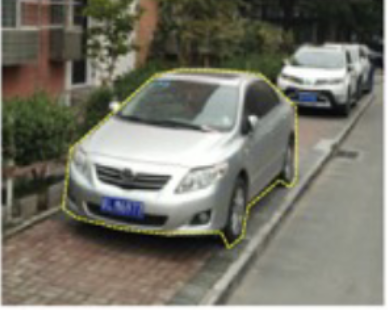
\includegraphics[width=\textwidth]{images/截屏2024-01-28 21.49.33.png}
  \end{column}
\end{columns}

\end{frame}

\subsection{Multi Images}

\begin{frame}[fragile]{Surpervision methods}

在多张图片的重建任务中,一个重要问题是:\textcolor{red}{Alignment}。

\begin{columns}
  \begin{column}{0.3\textwidth}
    存在的监督方式:
    \begin{itemize}
      \item 3D GT \quad \textcolor{red}{大多数时候难以获得,且不好优化}
      \item 2D GT
      \item depth
      \item course point
      \item no surpervision \cite{elbananiNovelObjectViewpoint2020}
      \item self surpervision
    \end{itemize}
  \end{column}

  \begin{column}{0.7\textwidth}
    \begin{figure}
      \includegraphics[width=\textwidth]{../storage/FKMEV2QK/image.png}
    \end{figure}
  \end{column}
\end{columns}

\end{frame}

\subsection{NeRF(2020)}

\begin{frame}[fragile]{Original Paper}
  
NeRF\cite{mildenhallNeRFRepresentingScenes2020}将场景表示成神经辐射场(Neural Radiance Fields),是一种隐式表达。

\begin{columns}
  \begin{column}{0.3\textwidth}
    \begin{itemize}
      \item 隐式表达场景,内存压力小
      \item 合成质量高
      \item \textcolor{red}{密度(density)}和\textcolor{red}{颜色(color)}
      \item 使用体渲染(volume rendering)
    \end{itemize}
  \end{column}

  \begin{column}{0.7\textwidth}
    \begin{figure}
      \includegraphics[width=\textwidth]{../storage/SCQXT534/image.png}
    \end{figure}
  \end{column}
\end{columns}

\end{frame}

\begin{frame}[fragile]{Improvement}
  
  \begin{figure}
    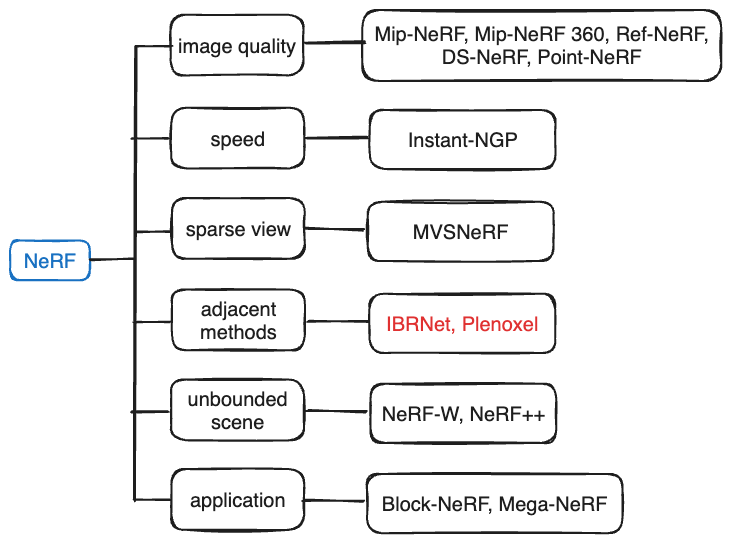
\includegraphics[width=0.6\textwidth]{images/NeRFImprovement.png}
  \end{figure}
  
\end{frame}

\begin{frame}[fragile]{Image Quality}

\begin{itemize}
  \item Mip-NeRF\cite{barronMipNeRFMultiscaleRepresentation},IPE
  \item Mip-NeRF 360\cite{barronMipNeRF360Unbounded2022},Mip-NeRF + unbounded scene
  \item DS-NeRF\cite{dengDepthsupervisedNeRFFewer2022},用SFM生成点云来监督depth
  \item Point-NeRF\cite{xuPointNeRFPointbasedNeural2022},预提取depth map和features来建立点云
\end{itemize}
  
改进思路:\textbf{数学原理、增强监督、特征增强、已存在的技术}

\end{frame}

\begin{frame}[fragile]{Speed}

  \begin{itemize}
    \item Instant-NGP\cite{mullerInstantNeuralGraphics2022} \quad 多分辨率编码、哈希函数、简化网络、球谐函数
  \end{itemize}

  \begin{figure}
    \includegraphics[width=0.7\textwidth]{../storage/TA9WBX5L/image.png}
  \end{figure}
    
  改进思路:\textbf{牺牲内存换取速度,插值法}
  
  \end{frame}

\begin{frame}[fragile]{Sparse View}

  \begin{itemize}
    \item MVSNeRF\cite{chenMVSNeRFFastGeneralizable2021} \quad 结合了MVSNet\cite{yaoMVSNetDepthInference2018}中提出的cost volume。
  \end{itemize}

  \begin{figure}
    \includegraphics[width=\textwidth]{../storage/WRPLJN97/image.png}
  \end{figure}
    
  改进思路:\textbf{参考前人工作,特征增强}
  
\end{frame}

\begin{frame}[fragile]{Adjacent Methods}

  \begin{itemize}
    \item IBRNet\cite{wangIBRNetLearningMultiView2021} \quad 相邻图片插值生成中间图片
    \item \textcolor{red}{Plenoxel}\cite{yuPlenoxelsRadianceFields2021} \quad 不使用神经网络,voxel表示场景,球谐函数表示颜色
  \end{itemize}

  \begin{figure}
    \includegraphics[width=0.5\textwidth]{../storage/9Z3XRRMK/image.png}
  \end{figure}
  
\end{frame}

\begin{frame}[fragile]{Unbounded Scene}
  这类场景需要分离物体与背景

  \begin{itemize}
    \item NeRF-W\cite{martin-bruallaNeRFWildNeural2021} \quad 解决灯光影响场景的问题
    \item NeRF++\cite{zhangNeRFAnalyzingImproving2020} \quad 分析并解决NeRF中的几何歧义性
  \end{itemize}

  \begin{figure}
    \includegraphics[width=0.6\textwidth]{../storage/TCTB7GQU/image.png}
  \end{figure}
  
\end{frame}

\begin{frame}[fragile]{Application}
  将NeRF应用到实际中

  \begin{itemize}
    \item Block-NeRF\cite{tancikBlockNeRFScalableLarge2022} \quad 结合了Mip-NeRF和NeRF-W来对大城市场景重建
    \item Mega-NeRF\cite{turkiMegaNeRFScalableConstruction2022} \quad 结合了NeRF++和NeRF-W来对无人机航拍的图片重建
  \end{itemize}

  解决思路:\textbf{将相应的工作应用到相应的场景中}
  
\end{frame}

\begin{frame}[fragile]{Conclusion of NeRF}

  Contributions:
  \begin{itemize}
    \item Plenoxel说明了NeRF的贡献不在于MLP,而在于使用\textcolor{red}{颜色和密度}来合成图片;
    \item 体渲染:\textcolor{red}{可微(differentiable)}的渲染方式。
  \end{itemize}
  Limitation:
  \begin{itemize}
    \item 速度慢
    \item 训练网络规模大
    \item 视觉质量的提升代价大
  \end{itemize}

\end{frame}

\section{3DGS(2023)}

\begin{frame}[fragile]{Contribution of 3DGS}

3DGS\cite{kerbl3DGaussianSplatting2023}是一种显式的表达方式,在速度和质量上都达到了SOTA。

\begin{columns}
  \begin{column}{0.3\textwidth}
    \begin{itemize}
      \item 基于点云(3D Gaussian)
      \item 球谐函数表示颜色
      \item 速度快、质量高
      \item 不需要神经网络
      \item 光栅化渲染
    \end{itemize}
  \end{column}

  \begin{column}{0.7\textwidth}
    \begin{figure}
      \includegraphics[width=\textwidth]{../storage/7S5X2Z2D/image.png}
    \end{figure}
  \end{column}
\end{columns}
  
\end{frame}

\begin{frame}[fragile]{Application}
  将3DGS应用到实际中,并评测

  \begin{itemize}
    \item SLAM \quad 确定全局地图信息,定位
    \item Dynamic Scene Modeling \quad 加入时间维度,4D
    \item Autonomous Driving \quad 使用3DGS重建场景
  \end{itemize}

  
\end{frame}

\section{Discussion and Conclusion}

\begin{frame}[fragile]{Discussion}

  一项新的研究灵感来源可以是:
  \begin{itemize}
    \item 前人工作 camP\cite{parkCamPCameraPreconditioning2023}
    \item 其他领域的工作
    \item 数学方法
    \item 发现本质
  \end{itemize}

\end{frame}

\begin{frame}[fragile]{Conclusion}

  本文从时间上的发展脉络,总结了在三维重建领域的关键技术及其发展。
  从单纯的摄影测量学到与计算机视觉、深度学习等领域相结合,三维重建正在变得越来越“智能化”。

  目前3DGS作为新视图合成中的SOTA方法,会是未来几年内的热门研究,然而在3年前兴起的NeRF将会有可能被其取代。

\end{frame}

\backmatter

\begin{frame}[t, allowframebreaks]{References}{\,}
\framesubtitle{\quad}
\tiny
  \bibliographystyle{apalike}
  \bibliography{reference}
\end{frame}


\end{document}
